\section{Experiments}
% ======================================================================

\problem{experiment\_log}{Experiment logging}{3}

\deliverable{Logging infrastructure code for your experiments and an experiment log for the problems below.}

\textbf{Tracking infrastructure.}
The training entry point, \texttt{cs336\_basics/train.py}, writes timestamped
messages to both the console and a per-experiment \texttt{train.log}.
Each run records its complete command-line configuration, dataset token counts,
training losses, validation losses, learning rates, elapsed time, throughput,
and checkpoint events. I use separate output directories and descriptive run
names to distinguish configurations. Training and checkpoints remain local;
optional Weights \& Biases (W\&B) tracking uploads metrics and configuration
when \texttt{--wandb-project} is supplied, with online and offline modes supported.

For the learning-rate experiments, I logged training loss every ten updates,
validated every 100 updates over 20 sampled batches, and saved a checkpoint
every 1,000 updates plus a final checkpoint on normal completion.
The logged training loss is the current minibatch loss, not an average over
the logging interval. W\&B records gradient steps, tokens processed, and elapsed
seconds together with each metric, so loss curves can be inspected against
steps or elapsed time. The following excerpt attaches these coordinates to
metrics before logging them:

\begin{lstlisting}[caption={Step, token, and elapsed-time coordinates for experiment metrics.}]
if metrics and run is not None:
    metrics.update(
        {
            "train/step": completed_steps,
            "train/tokens_seen": completed_steps * tokens_per_step,
            "time/elapsed_seconds": perf_counter() - started_at,
        }
    )
    run.log(metrics)
\end{lstlisting}

Timing uses \texttt{perf\_counter}; MPS/CUDA work is synchronized before
training timing samples to account for asynchronous execution. Throughput is
computed over the interval since the preceding training log, and can include
intervening validation and checkpoint overhead. Local timestamps also make
wall-clock interruptions visible. In the first short LR run, an automatic
system sleep caused an approximately nine-minute gap; subsequent runs used
\texttt{caffeinate -i}. W\&B's default loss axis is the gradient step, and
\texttt{time/elapsed\_seconds} is available as an alternative axis.

Checkpoints save model and optimizer states, the completed step count, and the
model configuration needed to reconstruct architecture variants. A resumed
invocation creates a new W\&B run and restarts elapsed-time accounting; it does
not automatically merge histories. Manually interrupted stability probes retain
their logs and any periodic checkpoints but do not receive a final checkpoint.
The learning-rate figures were exported directly from W\&B panels with
smoothing disabled. Panel filters separate short screening, full-budget
comparisons, and early stability probes; the horizontal axis uses
\texttt{train/step}. High-resolution PNG exports are included in this report.

\textbf{Experiment log to date.}
I used TinyStories on an Apple M4 with 16\,GB unified memory and MPS.
The following log separates runtime checks from convergence experiments;
detailed LR results and curves follow in Problem (\texttt{learning\_rate}).

\begin{table}[H]
    \centering
    \small
    \begin{tabular}{@{}>{\raggedright\arraybackslash}p{0.20\textwidth}
        >{\raggedright\arraybackslash}p{0.34\textwidth}
        >{\raggedright\arraybackslash}p{0.39\textwidth}@{}}
        \toprule
        Stage & Configurations tried & Observation / decision \\
        \midrule
        Throughput checks & Batch sizes 8, 16, 32; steps 51--100 measured
        & Approximately 7,880, 8,237, 8,218 tokens/s. Selected batch 16;
          these short checks do not establish convergence quality. \\
        \addlinespace
        Short LR screening & Peaks $3\times10^{-4}$, $10^{-3}$,
          $3\times10^{-3}$; 1,000 steps each
        & Final validation losses 2.6617, 2.3287, 2.5064.
          Selected $10^{-3}$ for full-budget investigation. \\
        \addlinespace
        Architecture smoke checks & Baseline, no RMSNorm, post-norm,
          NoPE, SiLU; 30 MPS steps each
        & All five passed training, validation, checkpoint checks,
          and reconstruction/forward checks. These are runtime checks,
          not formal ablation results. \\
        \addlinespace
        Full LR comparison & Peaks $5\times10^{-4}$, $10^{-3}$,
          $2\times10^{-3}$; 10,000 steps each
        & Final validation losses 1.6402, 1.5966, 1.6092.
          Retained $10^{-3}$ as the best tested full-budget setting. \\
        \addlinespace
        Early stability probes & Peaks 0.01, 0.03, 0.1, 0.3, 0.5;
          about 1,000 steps with a 10,000-step schedule
        & Increasingly poor learning; repeated loss explosions at
          0.3 and 0.5, with finite values and intermittent recovery.
          Stopped probes manually. \\
        \bottomrule
    \end{tabular}
    \caption{Completed checks and experiments. All LR experiments used seed 42;
    minimum LR was one tenth of peak LR.}
    \label{tab:experiment_log}
\end{table}

Full-budget architecture ablations are now complete: a fresh matched baseline
and four variants each trained for 10,000 updates (40.96M tokens), with fixed
validation windows and seed 42. Their configurations, results, and curves are
reported in Problems (\texttt{layer\_norm\_ablation}) through
(\texttt{swiglu\_ablation}). The text-generation analysis appears in
Problem (\texttt{generate}). The batch-size study remains incomplete and will
be reported after the remaining runs finish.


\newpage
\problem{learning\_rate}{Tune the learning rate}{3}

\textbf{(a) Search strategy and full-budget results.}

I used the Apple Silicon low-resource setting: each full run processed
$16\times 10{,}000\times 256=40{,}960{,}000$ tokens on TinyStories using MPS.
The model had a vocabulary of 10,000, four layers, width 512, 16 attention heads,
and SwiGLU hidden width 1,344, with pre-RMSNorm and RoPE. All runs used seed 42,
AdamW with $\beta=(0.9,0.999)$, weight decay 0.1, gradient clipping at 1.0,
and 100 warmup steps. The learning rate then followed cosine decay to one tenth
of its peak at the last planned step. Validation loss was averaged over
20 randomly sampled batches every 100 steps.

I first screened peak learning rates $3\times10^{-4}$, $1\times10^{-3}$, and
$3\times10^{-3}$ using independent 1,000-step runs (4.096M tokens each).
Their final validation losses were 2.6617, 2.3287, and 2.5064, respectively.
I then compared $5\times10^{-4}$, $1\times10^{-3}$, and $2\times10^{-3}$ in fresh
10,000-step runs to test both sides of the screening winner.
The screening and full runs used different cosine horizons; their final losses
therefore cannot be treated as equal-budget comparisons.

\begin{figure}[H]
    \centering
    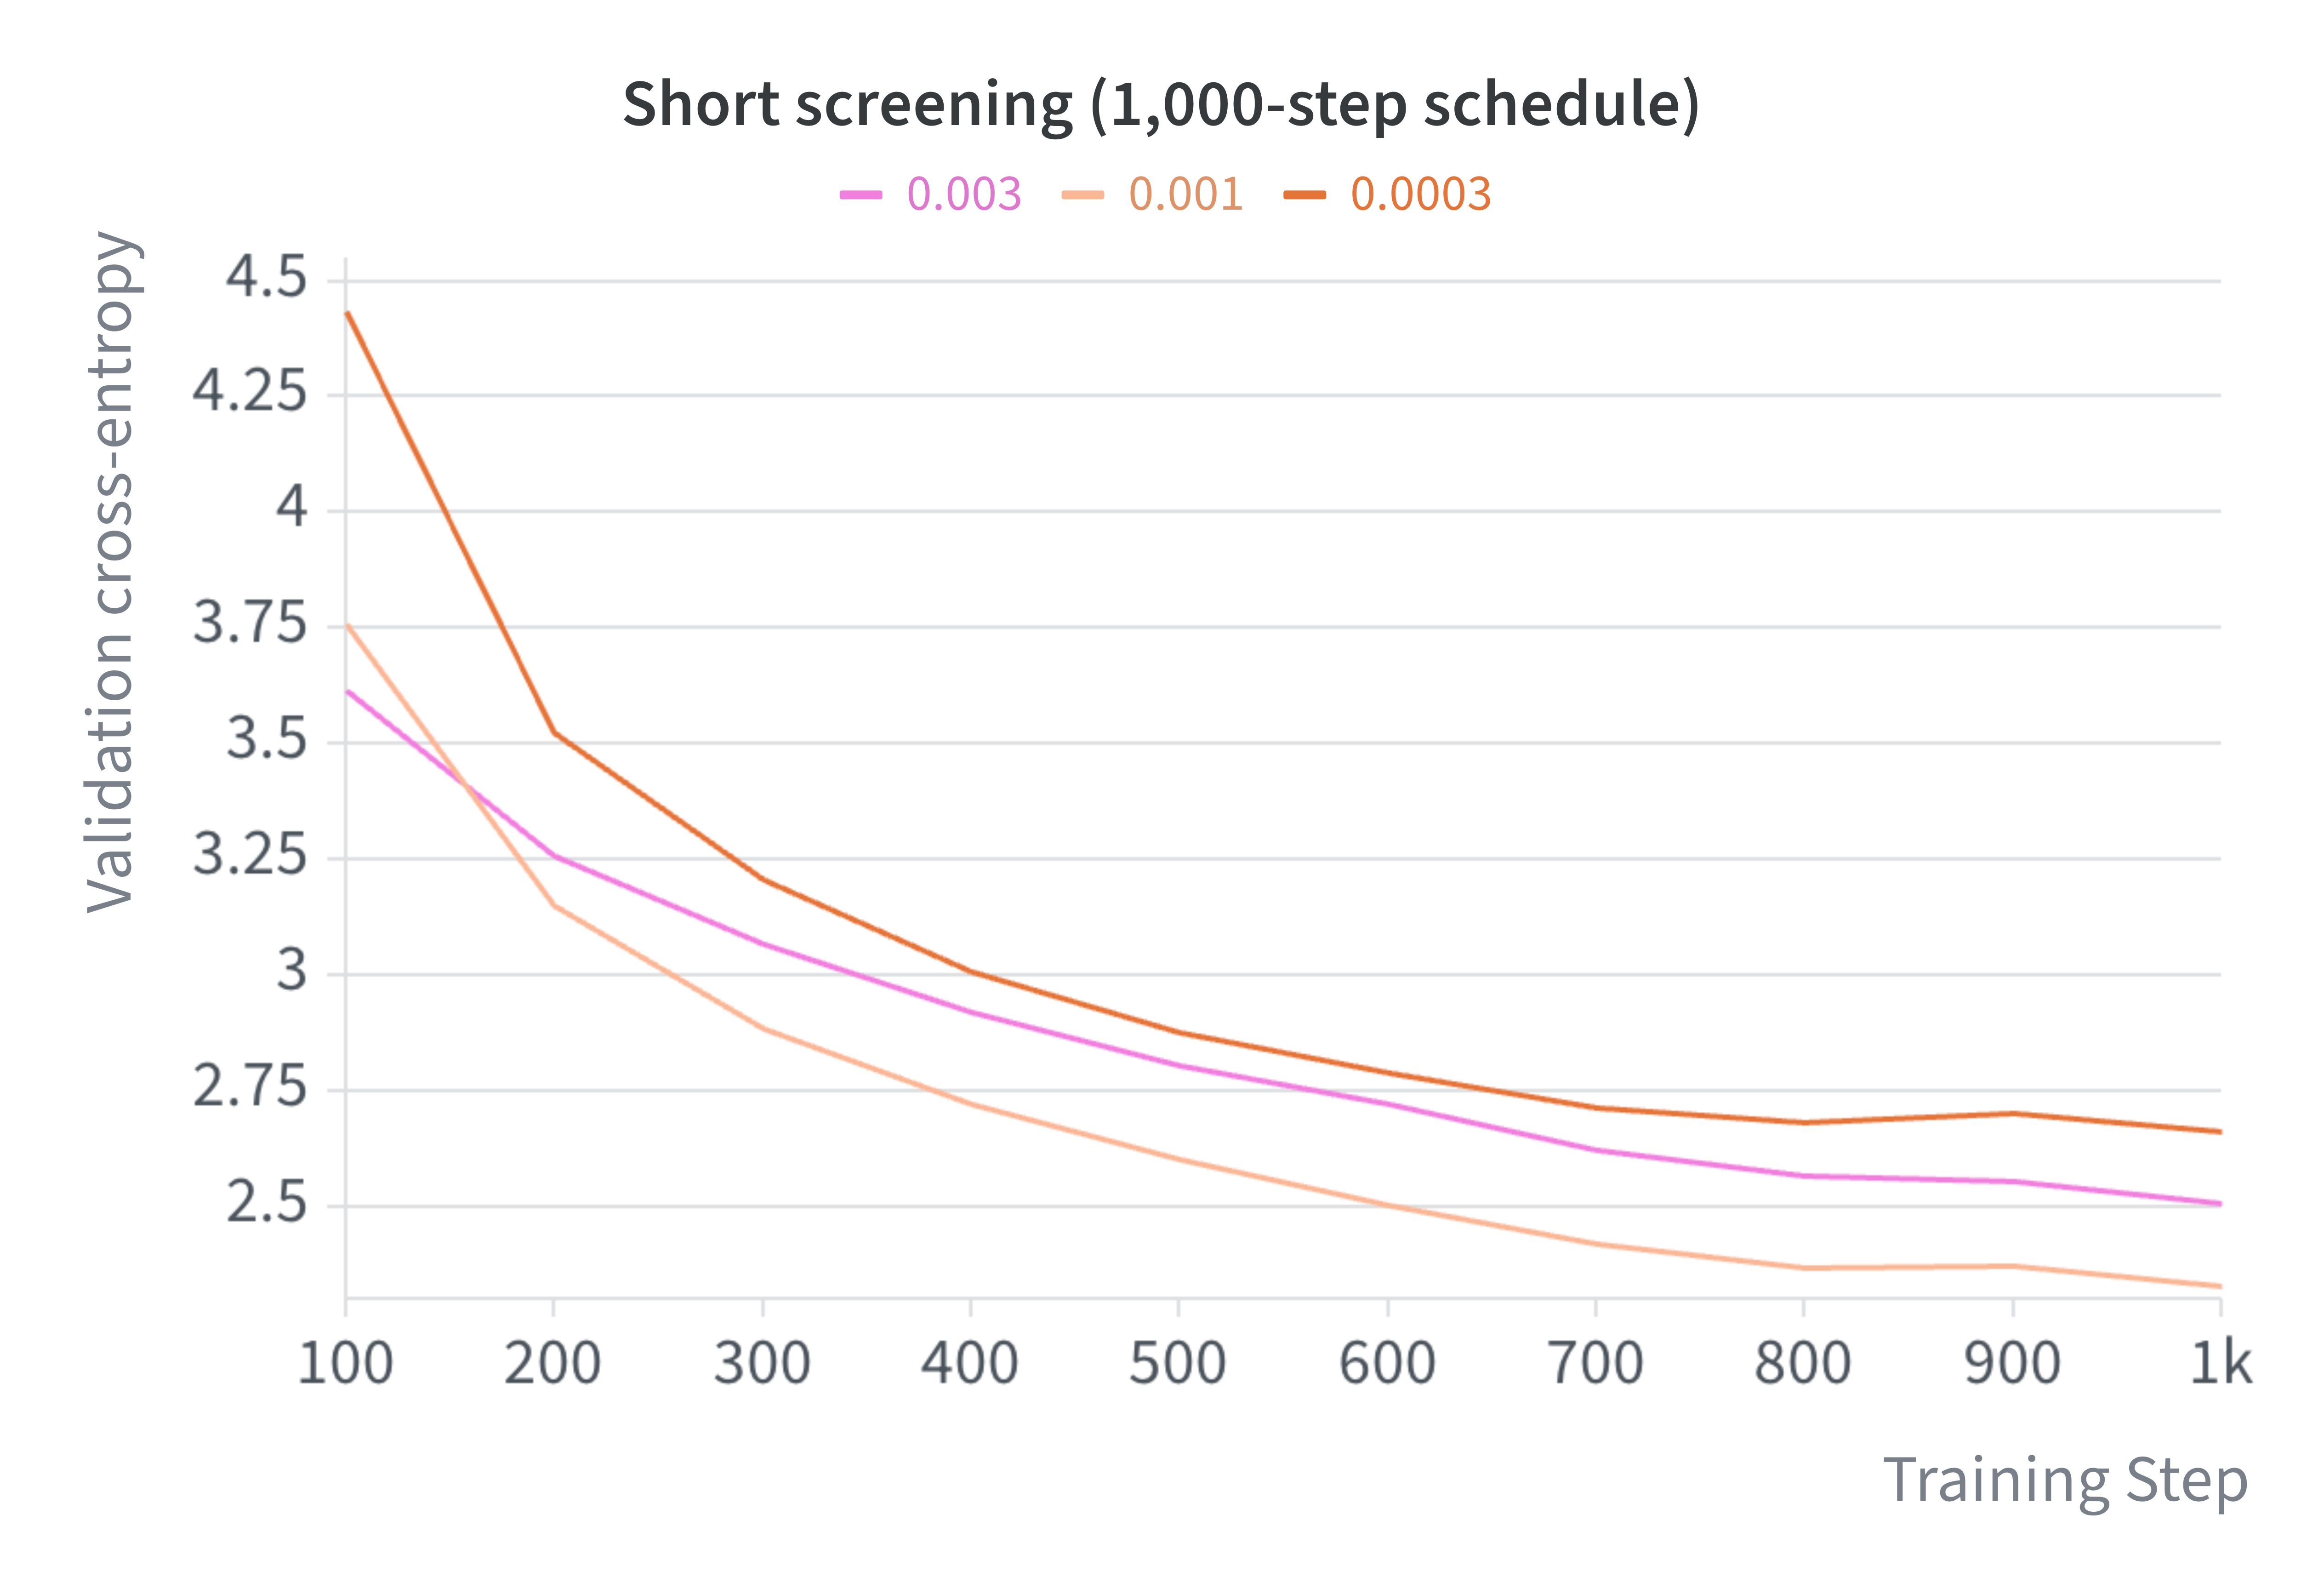
\includegraphics[width=0.49\textwidth]{figures/learning_rate_screening.png}\hfill
    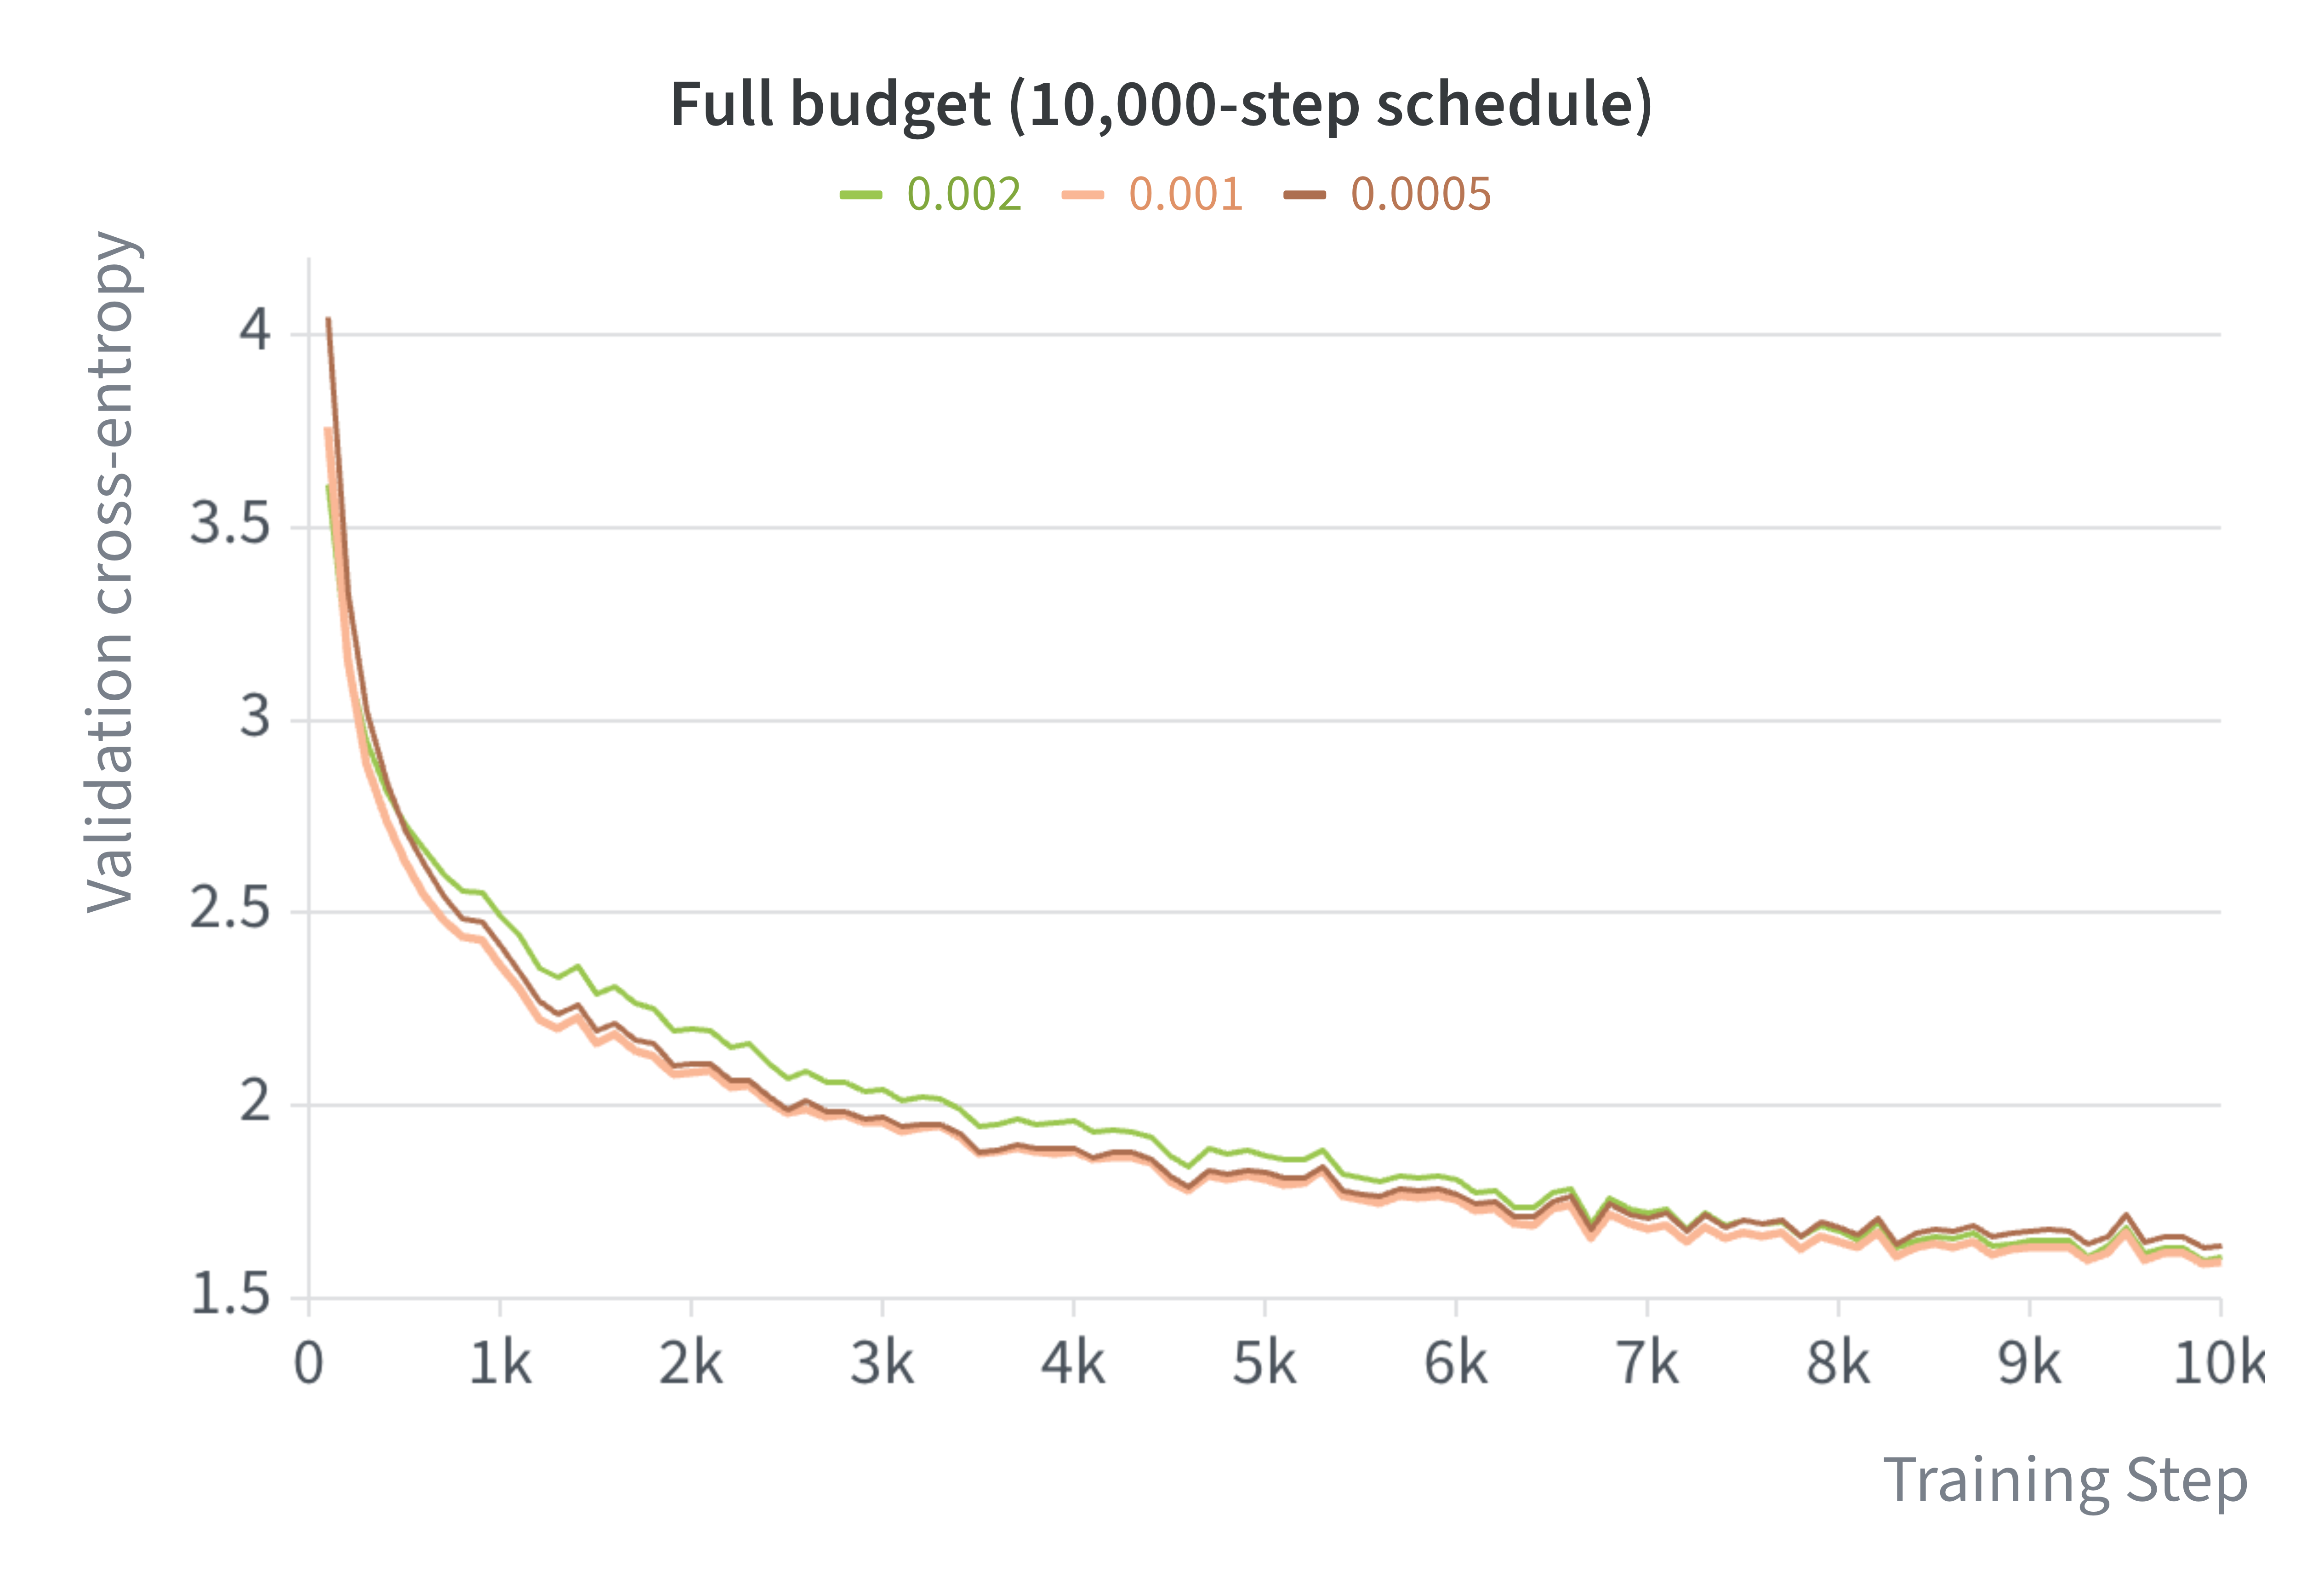
\includegraphics[width=0.49\textwidth]{figures/learning_rate_full_budget.png}
    \caption{W\&B validation curves for short screening (left) and
    full-budget comparisons (right), with smoothing disabled.
    Legends show peak learning rates. The low-resource validation target is 2.00.}
    \label{fig:lr_sweep}
\end{figure}

\begin{table}[H]
    \centering
    \small
    \begin{tabular}{@{}rrrrr@{}}
        \toprule
        Peak LR & Minimum LR & Final val loss & Best sampled val loss & Final PPL \\
        \midrule
        $5\times10^{-4}$ & $5\times10^{-5}$ & 1.6402 & 1.6343 & 5.16 \\
        $1\times10^{-3}$ & $1\times10^{-4}$ & \textbf{1.5966} & \textbf{1.5921} & \textbf{4.94} \\
        $2\times10^{-3}$ & $2\times10^{-4}$ & 1.6092 & 1.6010 & 5.00 \\
        \bottomrule
    \end{tabular}
    \caption{Equal-budget results after 10,000 steps (40.96M tokens).
    Final perplexity is $\exp(\text{final validation loss})$.}
    \label{tab:lr_results}
\end{table}

The best tested peak learning rate was $1\times10^{-3}$. It also had the lowest mean
validation loss over the last ten evaluations: 1.6188, compared with 1.6629
for $5\times10^{-4}$ and 1.6333 for $2\times10^{-3}$.
It outperformed these candidates at 100/100 and 98/100 corresponding evaluation
points, respectively. The final model reached validation loss 1.5966, meeting
the MPS low-resource target of 2.00; the best sampled loss was 1.5921 at step
9,900. I retained the final checkpoint and selected peak/minimum learning rates
$10^{-3}/10^{-4}$ for subsequent ablations. These are single-seed results over
three full-budget candidates, rather than evidence of a global optimum.

\newpage
\textbf{(b) High learning rates and stability.}

I increased the peak learning rate to $10^{-2}$, $3\times10^{-2}$, $10^{-1}$,
$0.3$, and $0.5$, keeping the other training settings fixed, including gradient
clipping. These fresh runs retained the 10,000-step cosine horizon and were
manually stopped at steps 1,040, 1,010, 1,080, 1,070, and 1,010, respectively.
Thus, these are early stability probes, not full-budget performance estimates.
Figure~\ref{fig:lr_divergence} compares their first 1,000 steps, during which
the post-warmup learning rates remained close to their peaks.

\begin{figure}[H]
    \centering
    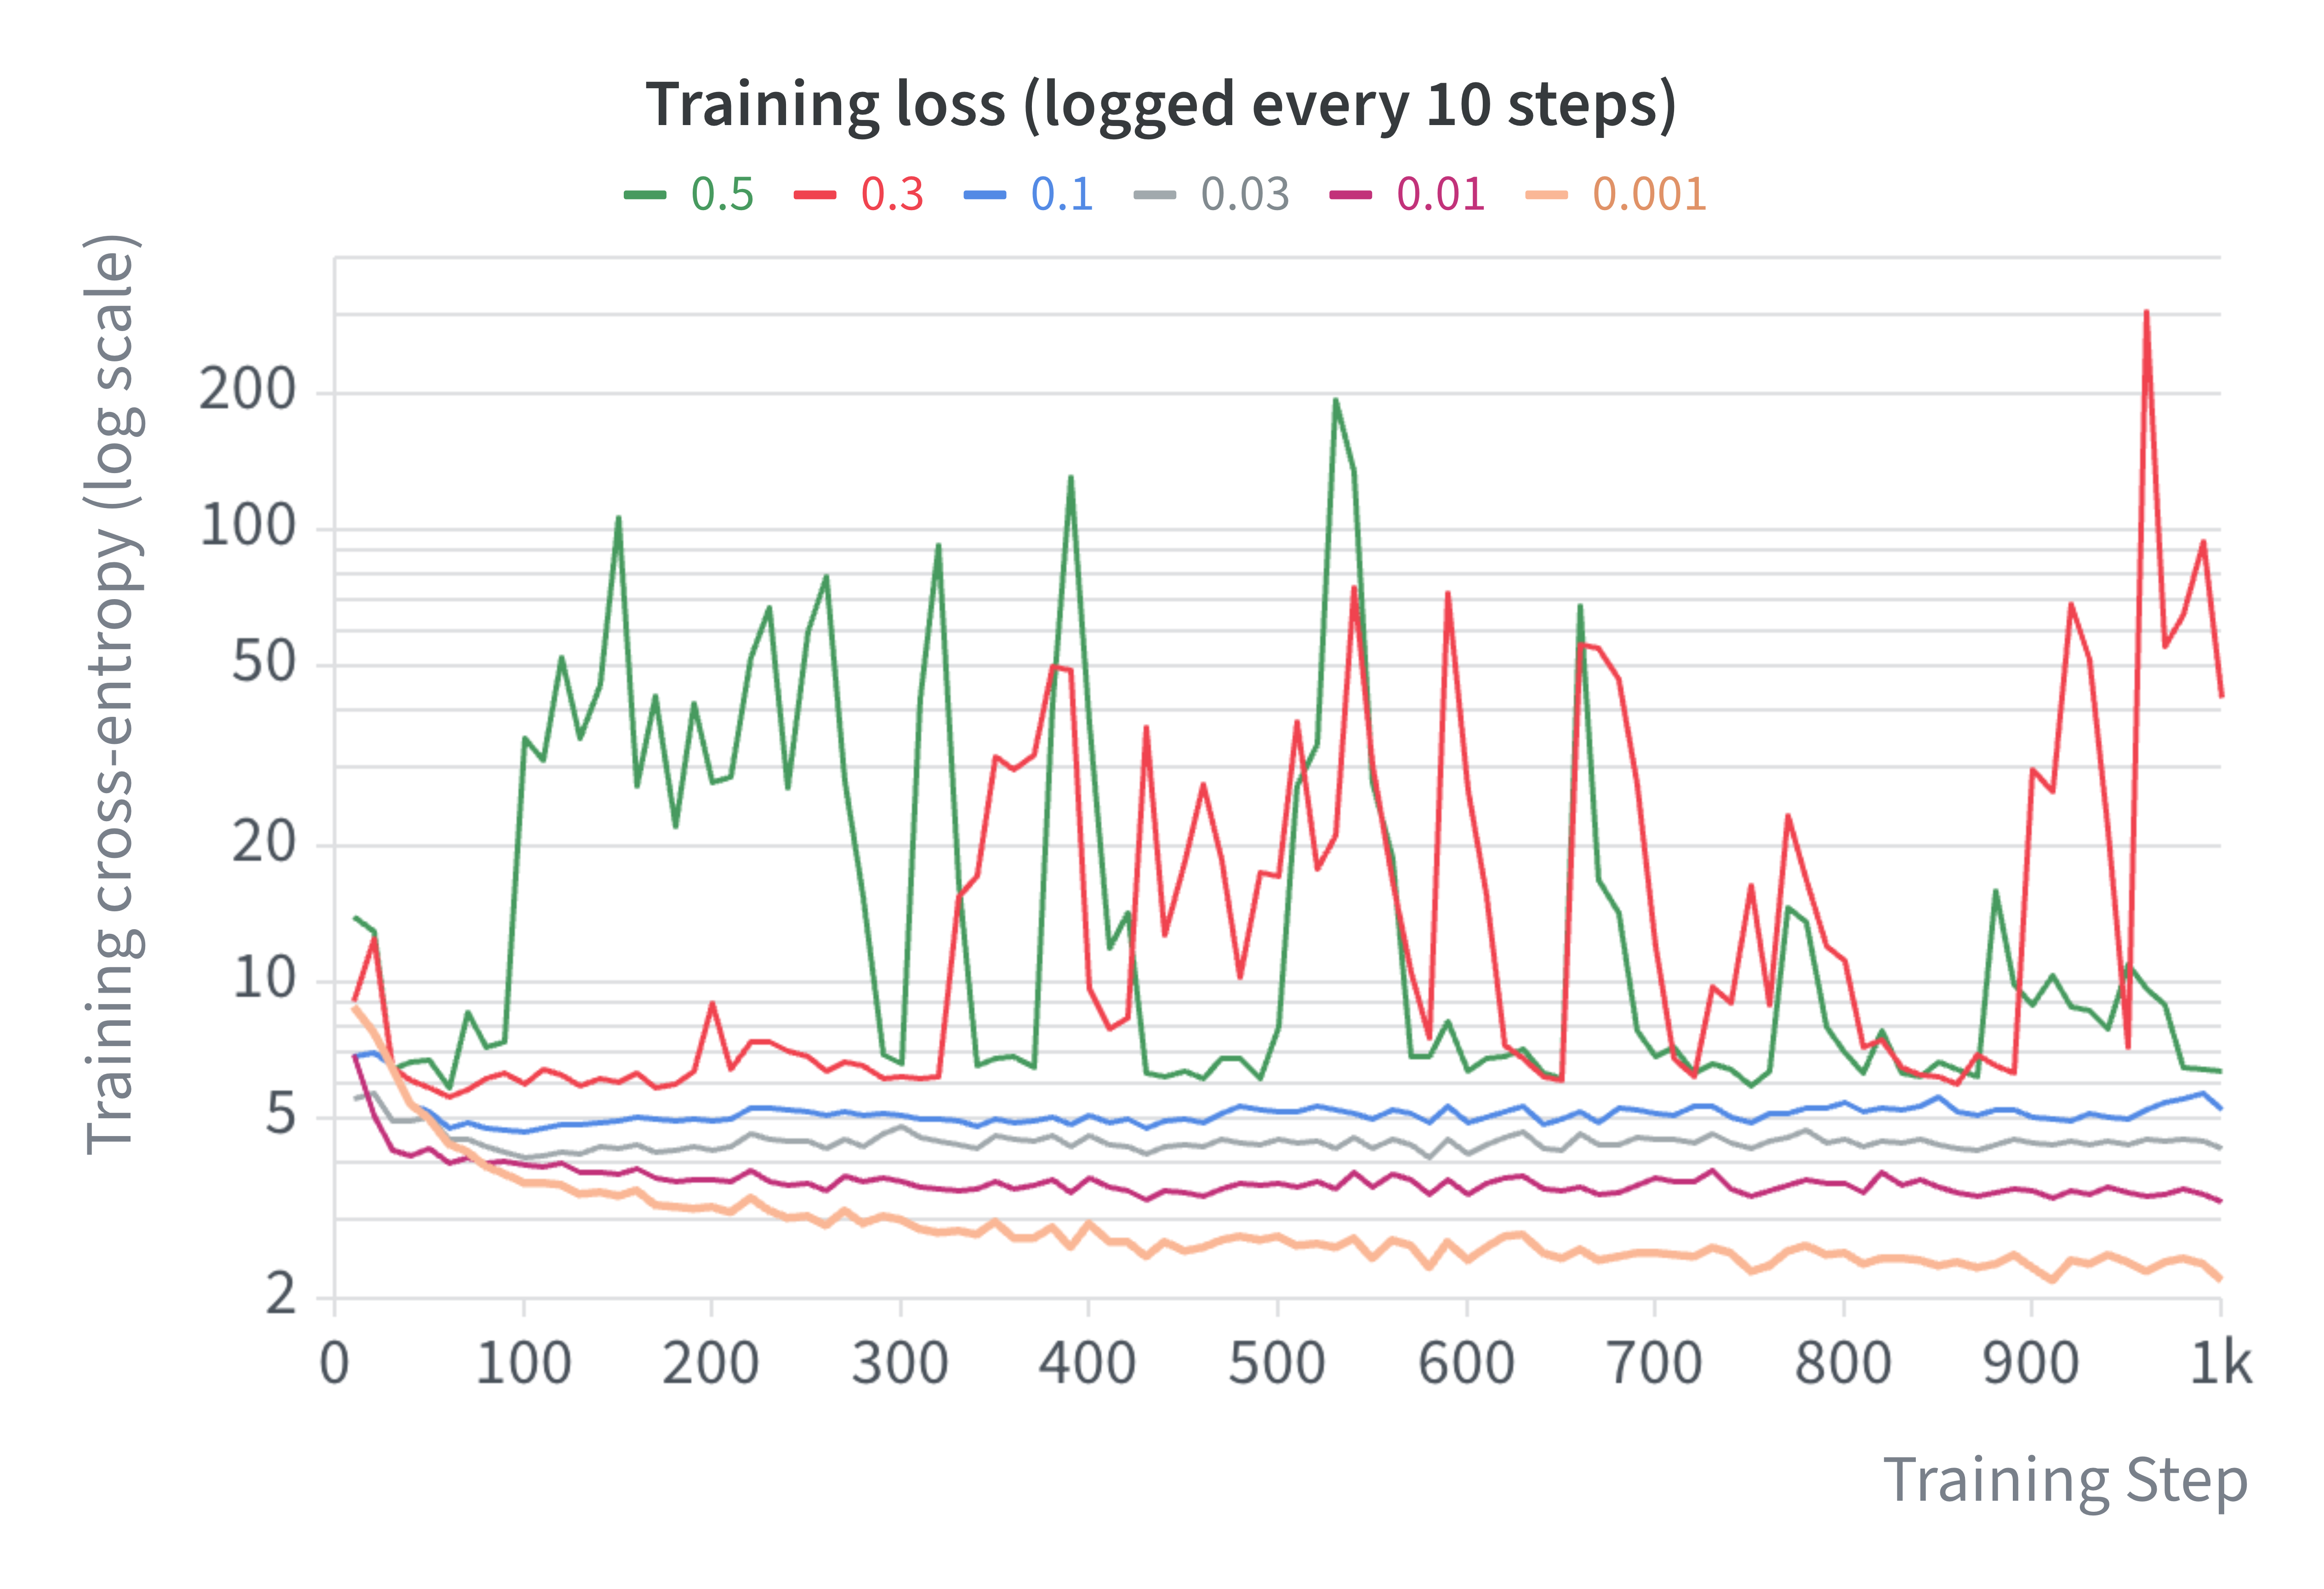
\includegraphics[width=0.49\textwidth]{figures/learning_rate_divergence_train.png}\hfill
    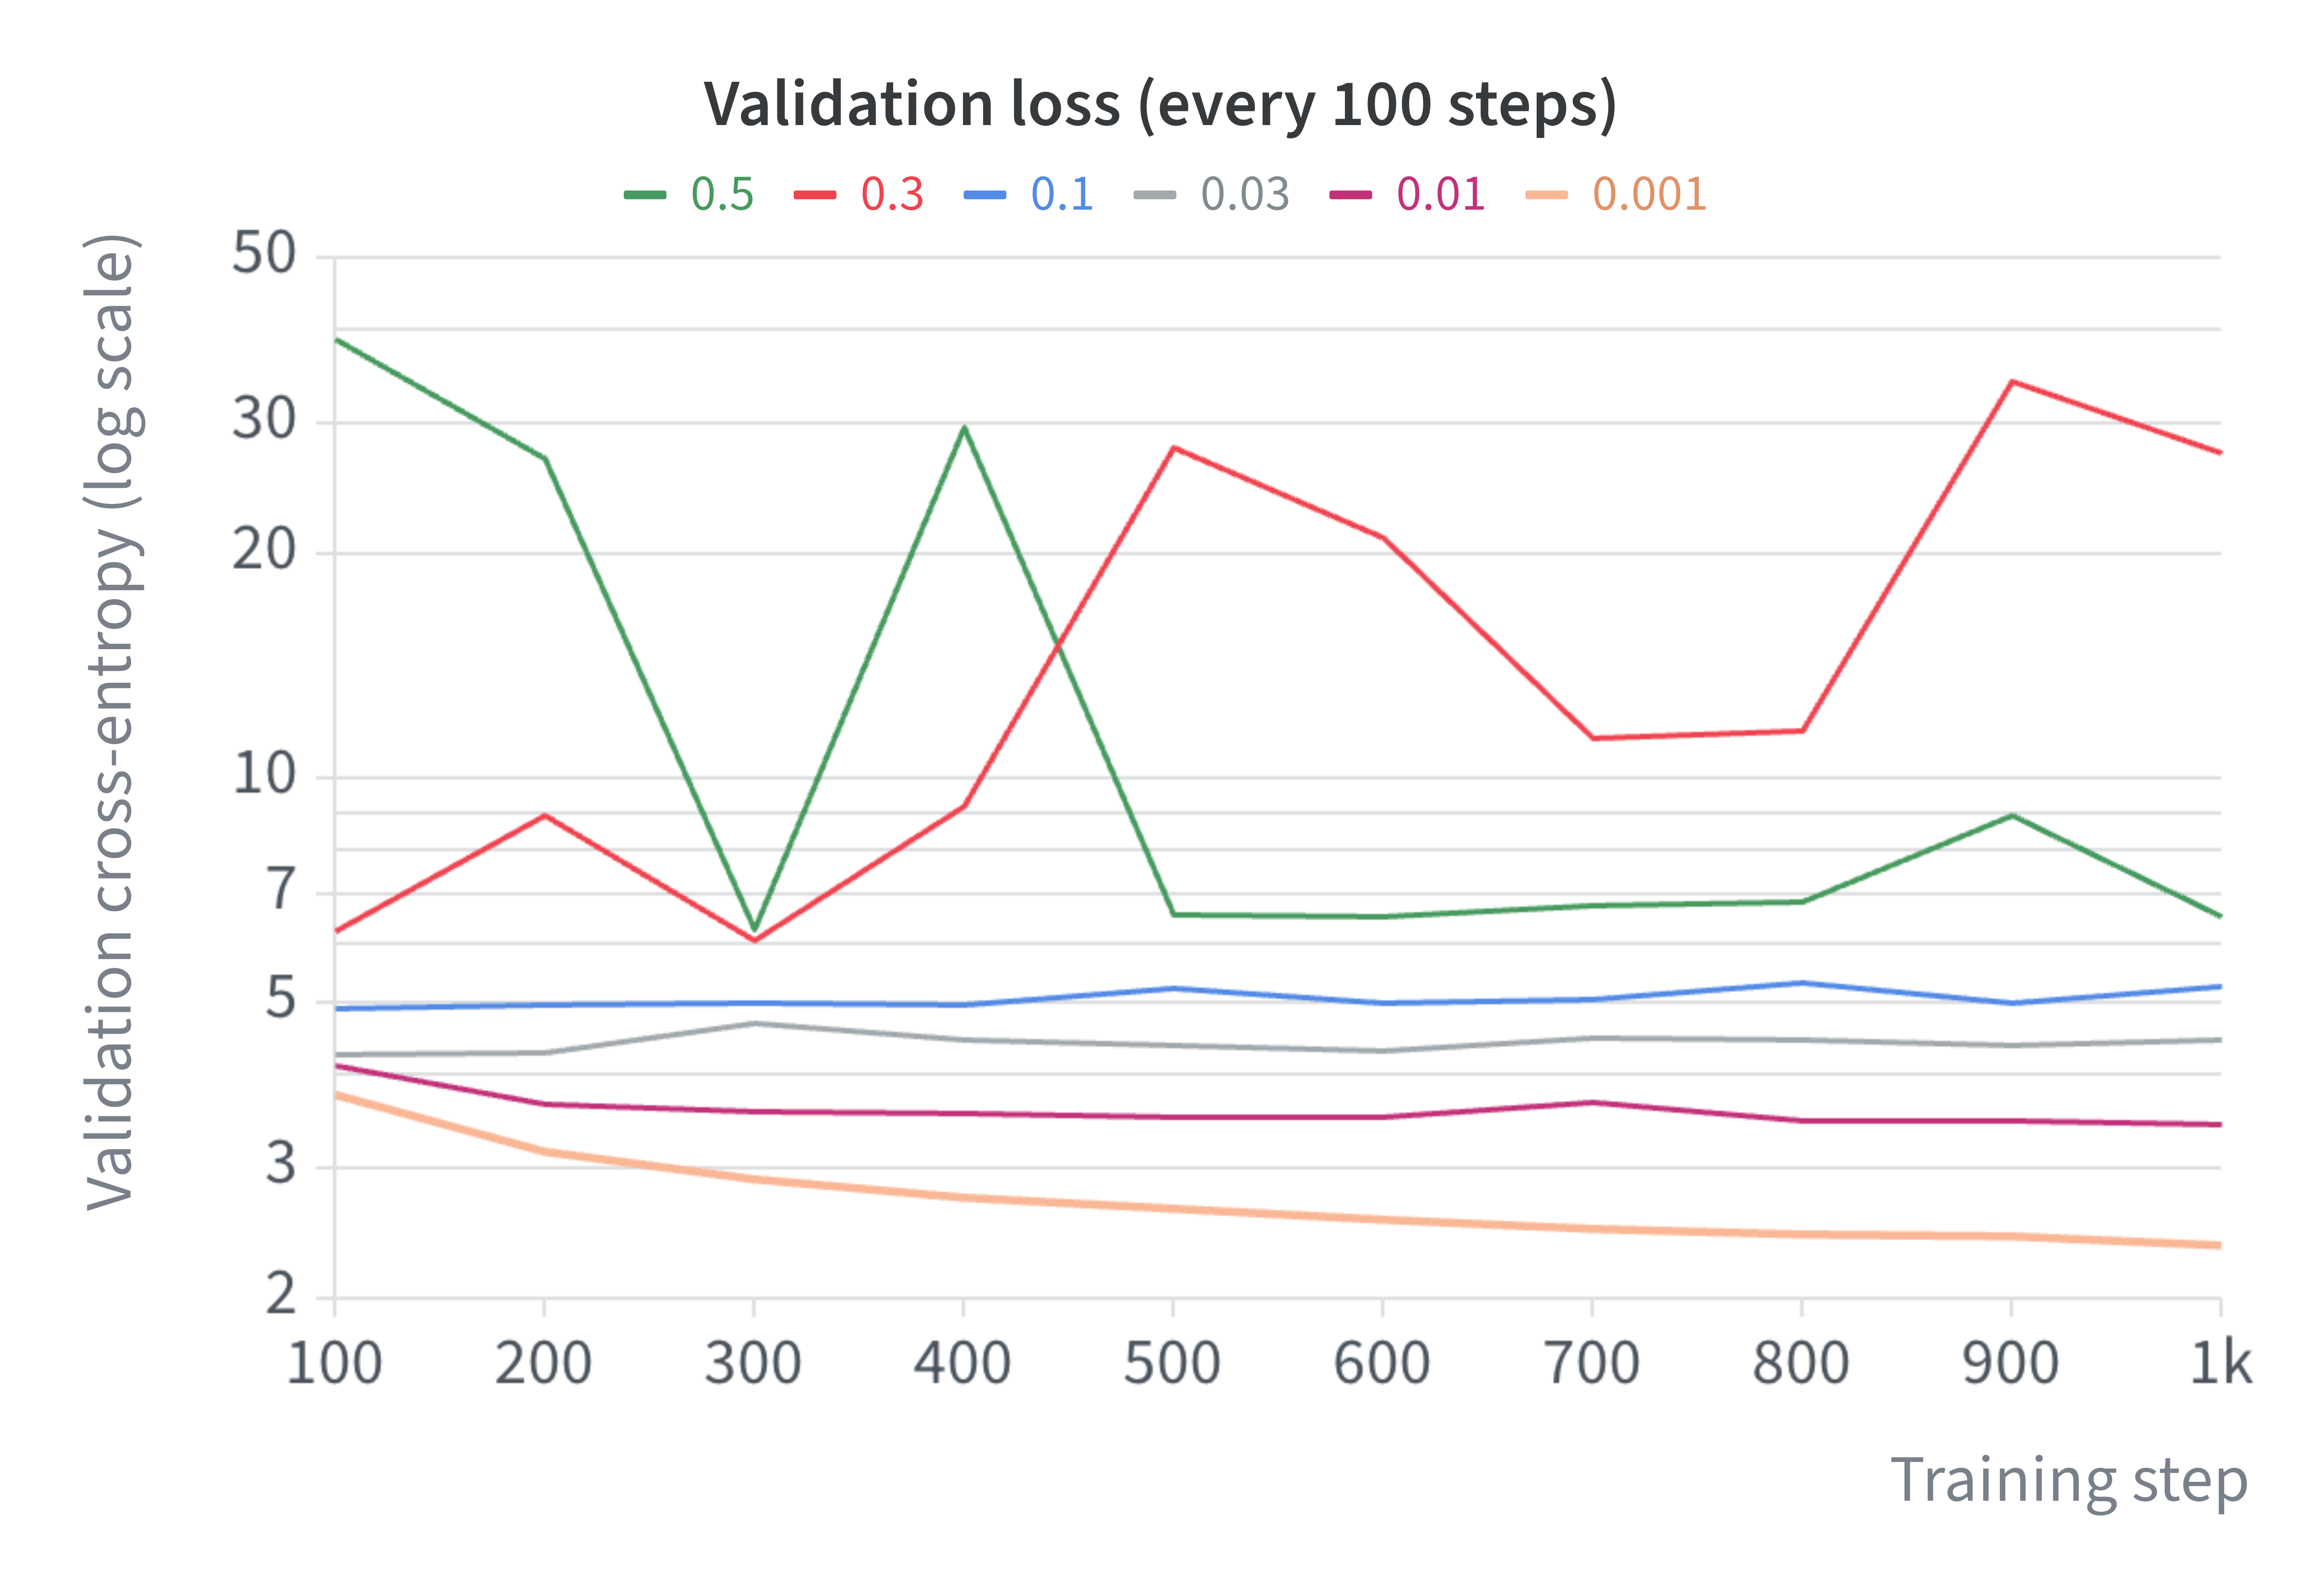
\includegraphics[width=0.49\textwidth]{figures/learning_rate_divergence_val.png}
    \caption{W\&B training (left) and validation (right) curves over the first
    1,000 steps, with smoothing disabled and logarithmic loss axes.
    Legends show peak learning rates; the $0.001$ curve is the full baseline
    restricted to this window. Warmup lasts 100 steps.}
    \label{fig:lr_divergence}
\end{figure}

\begin{table}[H]
    \centering
    \small
    \begin{tabular}{@{}rrl@{}}
        \toprule
        Peak LR & Val loss at step 1,000 & Observed behavior \\
        \midrule
        $10^{-3}$ & 2.3642 & Consistent improvement \\
        $10^{-2}$ & 3.4377 & Slow improvement \\
        $3\times10^{-2}$ & 4.4470 & High-loss plateau and oscillation \\
        $10^{-1}$ & 5.2528 & High-loss plateau and oscillation \\
        $0.3$ & 27.3223 & Repeated loss explosions \\
        $0.5$ & 6.5385 & Repeated loss explosions and recovery \\
        \bottomrule
    \end{tabular}
    \caption{High-LR probes compared at the same training step and token budget.}
    \label{tab:lr_stability}
\end{table}

The $10^{-2}$ run still learned, but much more slowly than the baseline;
$0.03$ and $0.1$ largely stalled. At $0.3$, training loss repeatedly exploded,
reaching a logged maximum of 305.5062 at step 960; validation loss reached
27.8814 at step 500 and 34.2393 at step 900.
At $0.5$, the logged training-loss maximum was 194.4761 at step 530, and
validation loss reached 38.9796 at step 100. These runs demonstrate optimization
divergence in the operational sense of repeated loss explosions and failure
to converge reliably. All logged values remained finite and losses sometimes
recovered: this is not evidence of NaN/Inf or monotonic, unbounded divergence.
The relatively low last validation loss for $0.5$ does not erase its earlier
instability.

In this search, increasing the learning rate beyond $10^{-3}$ did not accelerate
convergence: it first slowed learning and eventually caused severe instability.
The best full-budget candidate was well below the peaks showing loss explosions,
so these results do not support identifying it with a sharp ``edge of stability.''
The precise stability boundary was not located; the probes used one seed and
only about 1,000 steps, and the observed behavior depends on warmup, clipping,
and the other fixed settings.


\problem{batch\_size\_experiment}{Batch size variations}{1}

\deliverable{Learning curves for runs with different batch sizes.}

\begin{figure}[H]
    \centering
    % \includegraphics[width=0.8\textwidth]{figures/batch_size_experiment.png}
    \fbox{\parbox{0.8\textwidth}{\centering\vspace{2cm} Batch size experiment learning curves \\ \textit{(insert figure here)}\vspace{2cm}}}
    \caption{Learning curves for different batch sizes on TinyStories.}
    \label{fig:batch_size}
\end{figure}

\deliverable{A few sentences discussing your findings on batch sizes and their impacts on training.}

\textit{Findings:} % TODO: your findings


\problem{generate}{Generate text}{1}

\deliverable{Text dump of at least 256 tokens of text (or until the first \texttt{<eos>} token), and a brief comment on fluency.}

\textbf{Setup.} We used the final TinyStories baseline checkpoint trained
for 10,000 updates at batch size 16 (40.96M tokens), with peak/floor learning
rates $10^{-3}/10^{-4}$. Generation used MPS, seed 42, top-$p=0.9$, and a
limit of 256 new tokens, stopping earlier if EOS was sampled. The CLI omits
the terminal EOS from the displayed text. The prompt, checkpoint, seed, and
top-$p$ were fixed while temperature varied across $0.7$, $1.0$, and $1.3$.
Each text below includes the prompt.

\textbf{Generated text, temperature $0.7$.}
\begin{quote}
Once upon a time, there was a little girl named Lily. She loved to play outside in the snow. One day, she saw a big, pretty flower that was blooming in the sun. Lily thought the flower was very pretty.

Lily wanted to show her friends the flower. She took a big step and danced around. She saw her friends, the bees, and the bees. They all danced together, and Lily felt happy.

But then, a mean fox came to the garden. The fox wanted to take the flower from Lily and her friends. The fox was not nice to take the flower. He took the flower and ran away. Lily was sad and cried. She went back to her friends and told them about the fox. They all learned to be careful with the pretty flower and not let it hurt them.
\end{quote}

\textbf{Generated text, temperature $1.0$.}
\begin{quote}
Once upon a time, there was a little girl named Lily. She loved to play outside in the snow. One day, she saw a unique triangle in the snow. It was big and round. Lily was very happy and excited to play with it.

Lily picked up the triangle and put it on the ground. She played with it all day long. When it was time to go inside, she was tired but happy. So, she put the triangle in the snow and went inside to have some hot cocoa.

While she was outside, the unique triangle was starting to melt. It got bigger and bigger, and the triangle felt sad. Lily sat down under the snow and laughed. The triangle's face was gone, and the cone was gone.

From that day on, Lily and the unique triangle had many more fun playing in the snow. They made snow angels, even when it rained. And they always played in the snow together.
\end{quote}

\textbf{Generated text, temperature $1.3$.}
\begin{quote}
Once upon a time, there was a little girl named Lily. She loved to ask her mom to make some shampoo. One day, it was spoiled and was all one fun hair she could do.

Lily's mom told her to put a new red thread around like a lamp one by one. She said it would keep blue again, so Lily could have eleven wheel parties at once.

So every day. When the heel from put over all of the facereenening sizes of first, why hard about it now? But Lily resisted admiring it! They clapped for her, and she was so happy. She was able to put the oil over it every day.
\end{quote}

\textbf{Fluency and sampling.} Of these three samples, temperature $0.7$
produced the most coherent story and mostly grammatical sentences. However,
it repeated ``the bees'' and ended with a moral weakly connected to the plot.
At $1.0$, many sentences remained locally fluent, but the triangle was
described as round, grew while melting, and was followed by an unexplained
cone. At $1.3$, grammatical errors, unrelated phrases, and the malformed word
``facereenening'' made the story difficult to follow.

Two factors affect output quality. First, temperature changes the sampling
distribution: increasing it gives lower-probability tokens more weight,
potentially increasing variety while also admitting errors. Top-$p$ further
restricts the candidate set; it was held fixed here, so its effect was not
measured separately. Second, the learned model distribution matters: this
40.96M-token model can produce familiar story structures but still exhibits
repetition, semantic contradictions, and weak long-range consistency even at
the lowest tested temperature. The observed temperature ranking applies to
this prompt and seed; it does not establish a generally optimal temperature.
